\chapter{Lightweight Real-Time Feature Monitoring} \label{chap:my-work} \minitoc

\section{Approach A: Usage of outlier detection methods}
The first approach considered relied on outlier detection methods such as the ones presented in Section \ref{sec:outliers} and classified by the taxonomy in Figure \ref{fig:outlier-taxonomy}. This straightforward approach works with either subsequence or point outlier detection methods to analyze the streaming sliding window and produce data pattern shift alerts.

\subsection*{How}

Using point outlier detection methods, the main idea is to keep track of the rate of point outliers detected. For instance, keep track of how many outliers were alerted in the past hour. The decision to alert for a data pattern shift of the system would be made when comparing this rate of point outliers detected in the past hour with a user-defined threshold $\alpha$. On the other hand, using subsequence outlier detection methods would allow us to report the whole sliding window as an outlier. 


\subsection*{Challenges}
The analyzed outlier detection algorithms in Section \ref{sec:outliers} were deemed unfit for our use-case due to one or more of the following: \textit{(a)} high memory consumption, \textit{(b)} high time complexity, \textit{(c)} "memory loss" and \textit{(d)} obfuscated insights.

In our lightweight real-time solution we need constant time complexity to process events one by one in real-time. Because our system is not mission-critical, we also want the solution to be as lightweight as possible, which means techniques that grow linearly with window size are not a good fit. Therefore, most of the outlier detection methods presented become unfit for our use due to high memory consumption and time complexity. Some of the methods discussed also suffer from what we call \textit{"memory loss"}: they lose track of the reference window or normality period. In other words, the algorithms are online learners, meaning they adapt to the underlying statistics of the data stream. While in some scenarios this is a much-needed feature, in our use-case it is not. How clear the alerts and insights retrieved from the methods are, is also an important property. Some outlier detection methods use Machine Learning (ML) techniques to produce alerts, which makes it harder to explain to a system administrator why an alert was raised and what changed.

\subsection*{Conclusion}
The outlier detection methods reviewed in Section \ref{sec:outliers} were discarded as viable solutions to our problem because of the aforementioned problems of memory and/or time complexity, \textit{"memory loss"} and non-explainable alerts.

We concluded that employing outlier detection methods was not the best course of action and put aside this approach.

\section{Approach B: Thresholding aggregation values}
This second approach focus on building an aggregation snapshot of the reference period to compare with streaming aggregation values and alert if the difference between both surpasses a threshold $\alpha$.

\subsection*{How}

In this approach we compute sliding window aggregations and compare the aggregations’ current state versus an initial reference, reporting a shift when the difference is substantial. For instance, consider the case where we monitor one single feature or variable \textit{x}. Assume we define the set of aggregations to compute the mean of \textit{x} and its standard deviation. Also assume we save the reference window and maintain a sliding window and the average and standard deviation aggregations for \textit{x} efficiently. As seen in Figure \ref{fig:approach2-initial-state}, the initial mean and standard deviation values for \textit{x} presented in the reference window are of 5 and 1, respectively. Later on, in \textit{Window 1}, we see the same values for the mean and standard deviation, of 5 and 1, respectively. This represents a \textit{normal} case where no alert is produced.

\begin{figure}[!htb]
    \begin{center}
      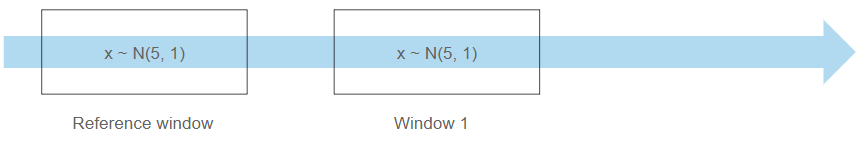
\includegraphics[scale=0.65]{figures/approach2-normality.png}
      \caption[]{Normal state for feature \textit{x} in window 1}
      \label{fig:approach2-initial-state}
    \end{center}
\end{figure}


In Figure \ref{fig:approach2-alert-state}, after further sliding steps of our sliding window, we obtain \textit{Window 2}. In \textit{Window 2}, the mean and standard deviation aggregation values change from 5 and 1 to 12 and 6, respectively. In this case, we would measure the difference between the sliding window aggregations and the reference window ones and if above a certain threshold raise an alert. For example, if we used a threshold of $\alpha$ = 6, we would raise an alert, as at least one sliding aggregation, in this case the mean, would differ of at least $\alpha$ when compared to the reference value.

\begin{figure}[!htb]
    \begin{center}
      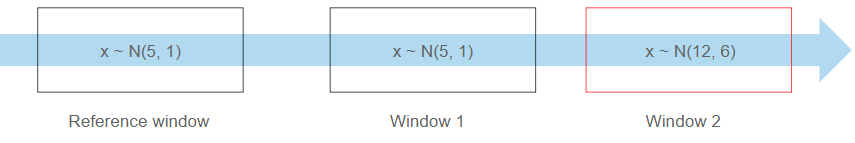
\includegraphics[scale=0.65]{figures/approach2-alert.png}
      \caption[]{Alert state for feature \textit{x} in window 2}
      \label{fig:approach2-alert-state}
    \end{center}
\end{figure}

\subsection*{Challenges}
The first issue with this approach is that generic sliding window aggregation algorithms grow linearly in space regarding window size, such as Recalculate-From-Scratch and Subtract-On-Evict presented in Section \ref{sec:back-swag-algs}, Two-Stacks has seen in Section \ref{sec:2stacks} and DABA in Section \ref{sec:daba}. Another challenge when using this approach is defining the set of aggregations to compute at feature/variable level that represent the system state well enough for comparison of reference and streaming periods and change detection. 

Exponential Moving Averages (Section \ref{sec:emas}), Probabilistic Data Structures (Section \ref{sec:pds}) and their sliding window implementations (Section \ref{sec:sliding-pds}) can be used to solve the first issue and reduce the linear memory complexity of the system relative to sliding window size. 

However, there is no trivial solution for the second challenge. Defining the set of aggregations to use does not have a straightforward solution. To illustrate this problem, consider both time-series show in Figure \ref{fig:approach2-timeseries}.
 
\begin{figure}[!htb]
    \begin{center}
      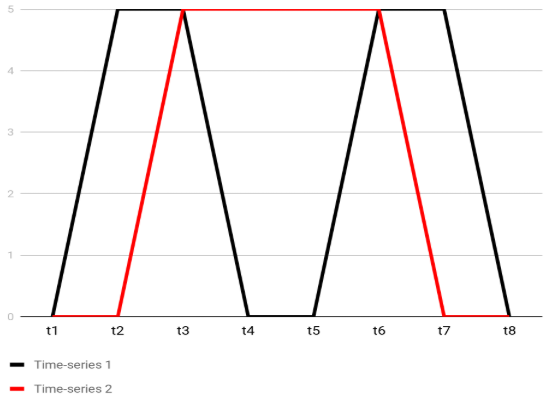
\includegraphics[scale=0.7]{figures/approach2-timeseries.png}
      \caption[]{Two different time-series with same max, min, mean and standard deviation}
      \label{fig:approach2-timeseries}
    \end{center}
\end{figure}

\textcolor{red}{NOTE TO MOPS: You commented here, but arent EMAs senseitive to time correlations? Since we put lower weights on older events, the order matters (while in a sliding window every event has the same weight (1))}
Both time-series 1 and 2 have the same maximum, minimum, mean and standard deviation values for the time-based window between \textit{t\textsubscript{1}} and \textit{t\textsubscript{8}}. Hence, if our set of aggregations chosen were the maximum, minimum, mean and standard deviation, we would not differentiate between these two different time-series.

\subsection*{Conclusion}
This approach requires efficient sliding window aggregation state maintenance, which can be done using sliding window probabilistic data structures and/or exponential moving averages. However, the need to choose a set of aggregations to use and the deviation threshold itself ultimately led us to discard this approach.


\section{Proposed method: Feature Distribution Monitoring} \label{sec:ft-monitoring}

A data stream is a continuous collection of events. Each event is timestamped and contains multiple fields. In the context of this Thesis, each of the event's fields are time-dependent variables named features. They can be thought of as columns in a traditional relational database table. Our goal is to detect data pattern shifts for each feature in an online fashion. Such shifts will be measured between a reference period versus the observed reality during the streaming phase. Figure \ref{fig:timelines} shows the separated reference and streaming timelines.

\begin{figure}[!htb]
    \begin{center}
      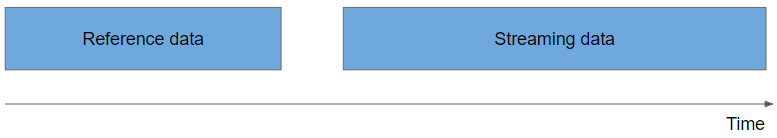
\includegraphics[scale=0.4]{figures/timeperiods.png}
      \caption[]{Reference and Streaming timelines}
      \label{fig:timelines}
    \end{center}
\end{figure}


We do not need to directly compare the entire window contents of the reference and sliding window periods. The latter would require storing all window contents hence making the memory consumption grow linearly with sliding window and/or reference period size. Instead, we want to use a  \textit{(a)} constant in memory aggregation that can be \textit{(b)} incrementally maintained during the streaming phase. Additionally, we want a streaming aggregation that \textit{(c)} reliably encodes the distribution of each feature. 

Histograms are a representation of the distribution of numerical or categorical data thus being ideal to encode the distribution of feature values, satisfying \textit{(c)}. Histograms require the storage of a fixed-size list of bins and a corresponding fixed-size list of counts per bin for ever growing volumes of data, satisfying property \textit{(a)}. Adding or removing an element to the histogram aggregation is tantamount to determining the correct bin and adding or subtracting one, respectively, thus satisfying property \textit{(b)}. However, computing an histogram aggregation over a sliding window of size $W$ implies storing all $W$ elements in memory to know the element to remove after a new one is inserted. This violates our constant in memory property \textit{(a)} which is why we chose to use the Exponential Moving Averages (EMAs) analyzed in Section \ref{sec:emas}. EMA-like histograms computed over sliding windows do not require the storage of window contents. An EMA-like histogram is \textit{(a)} constant in memory, \textit{(b)} maintained in real-time and \textit{(c)} encodes the distribution of each feature values. EMA-like histograms are further explained in Section \ref{sec:ema-hist}.

Since the reference window is static, \textit{i.e.}, it is not a sliding window, we can use exact histogram aggregations. Hence, for each feature, we build an exact reference histogram aggregation. On the other hand, in streaming, we use one EMA-like approximate histogram aggregation per feature (Figure \ref{fig:timelines-hists}).


\begin{figure}[!htb]
    \begin{center}
      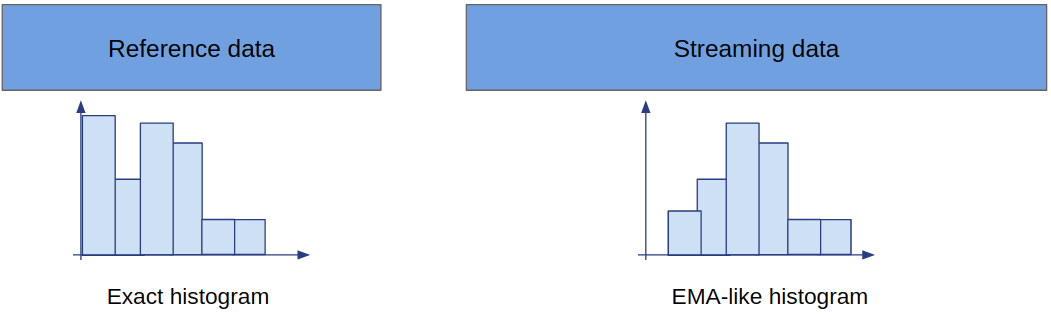
\includegraphics[scale=0.4]{figures/timelines-hists.png}
      \caption[]{Reference and Streaming timelines and corresponding histogram aggregations}
      \label{fig:timelines-hists}
    \end{center}
\end{figure}


To compare each feature's reference and sliding window histogram aggregation we need a measure of divergence. We chose to use the Jensen–Shannon Divergence (JSD) \cite{JSD} but other statistical tests are possible such as Kolmogorov-Smirnov or Wasserstein. A more thorough analysis on some statistical tests and why we chose to use the JSD is performed in Section \ref{sec:whyjsds}. Given a divergence value for the two aggregations (reference and sliding window ones) we need a measure of normal statistical fluctuations. Since we assume a reference period as the normal state we can find out the normal distribution for the divergence by sampling smaller windows of data from the reference period in a batch analysis. This allows us to define a threshold based on percentiles, which gives an estimate for the probability of a certain value occurring, rather than using a constant hand picked threshold for the divergence value (details in Section \ref{sec:sampling-batch}). 


We devise a two-phase method. The first phase relies on a batch analysis that, for each feature, builds a reference histogram and computes the distribution of divergence values (details presented in Section \ref{sec:batch-phase}). The second phase (detailed in Section \ref{sec:stream-phase}) focus on efficiently updating the sliding window histogram for each feature and periodically performs a divergence test between the static reference aggregation and the sliding one, alerting for changes if need be. The proposed method currently works only for numerical features, that is, only for event fields or variables that are of numeric type, but can be extended to other types.


\subsection{Exponential Moving Average based histogram} \label{sec:ema-hist}
As stated, we compute histogram aggregations for the reference and sliding windows. The computation of the reference histogram is done once in batch and hence an exact histogram can be computed. However, the sliding window histogram is an EMA-like histogram to ensure that we are able to encode the feature distribution with constant space complexity and maintain it in real-time.

In Section \ref{sec:emas} we discussed Exponential Moving Averages (EMAs) and how they emulate a sliding window without actually storing window elements....

\textcolor{red}{TODO: complete this after EMAs in background are corrected}

\subsection{Batch analysis phase} \label{sec:batch-phase}
\textcolor{red}{TODO: add some pseudocode}

The goal of the batch phase will be to build our reference aggregation for each feature and get to know the distribution of divergence or distance values between the reference and the sliding window aggregations. In other words, we:

\begin{enumerate}
    \item obtain a reference histogram for each feature using all data in the reference period
    
    \item then compute the distribution of distances between the reference histogram and the sliding window histogram by computing the distance (or divergence value) between the reference histogram and various samples of sliding window histograms
\end{enumerate}

This distribution of values can then later be compared to a given value of divergence for a single sample to find out how probable that value is to occur (if it is very low an alert may be raised).

\subsubsection*{Building the reference histogram for each feature}

First, for each feature, we compute the reference histogram from the reference period dataset. This is an exact histogram aggregation. When building it we ensure the histogram has equal counts (or equal height) for all bins which often results in different sized bins. We make no assumption on the dataset distributions and hence use equal height histograms because they adjust better to wildly varying ones. Equal height means we have more bins covering very dense regions (regions with many data points) and fewer bins in lower density regions. 

\begin{figure}[!htb]
    \begin{center}
      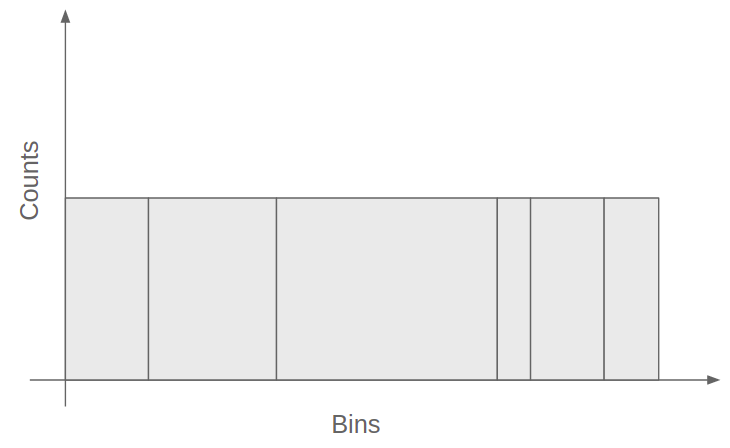
\includegraphics[scale=0.4]{figures/ref-hist.png}
      \caption[]{Reference equal-height histogram}
      \label{fig:ref-hist}
    \end{center}
\end{figure}


\subsubsection*{Finding the distribution of distances for each feature} \label{sec:sampling-batch}

Secondly, we aim to build the histogram that encodes the distribution of expected distance values, to later on threshold the observed distance values during the online phase. To that end, we make \textit{S} samples of transactions, each with the same tuple-based size of the sliding window we will use in streaming. Each sample is a contiguous block of transactions, thus preserving the order of transactions and the time-dependency property of a time-series. 

For each sample, and for each feature, we compute the approximated histogram using the bins computed for the reference histogram (Figure \ref{fig:ref-hist-bins}). We also add two extra bins that will cover the region to the left and to the right of our histogram, respectively. In other words, we add a bin that covers the region between $-\infty$ and our first bin and another that covers values from the last bin to $+\infty$. This way, observed values outside of the reference period will be placed in these special bins, either left or right.

\begin{figure}[!htb]
    \begin{center}
      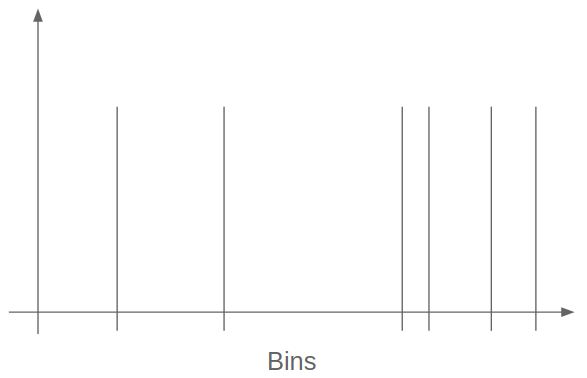
\includegraphics[scale=0.4]{figures/ref-bins.png}
      \caption[]{Reference equal-height histogram}
      \label{fig:ref-hist-bins}
    \end{center}
\end{figure}

Each of the histograms is an EMA-like histogram. An EMA-like histogram is essentially a collection of EMA-counts, as described in Section \ref{sec:ema-hist}. Each sample is processed event by event and a discount factor is applied per event, thus building an approximated histogram aggregation, using the reference bins, for each feature of that sample. We compute multiple sample histograms to encode distributions over smaller time periods that may exist within the large reference period. We use an approximated histogram to mimic the target approximated histogram we will incrementally maintain in the streaming environment.

For each feature, we have now \textit{S} histograms, one for each sample. For each of the \textit{S} histograms, we compute the distance between it and the reference histogram. Figure \ref{fig:compute-sample-distances} illustrates this process as we apply our distance function for each sample histogram and the reference histogram, obtaining \textit{S} distance measurements.

\begin{figure}[!htb]
    \begin{center}
      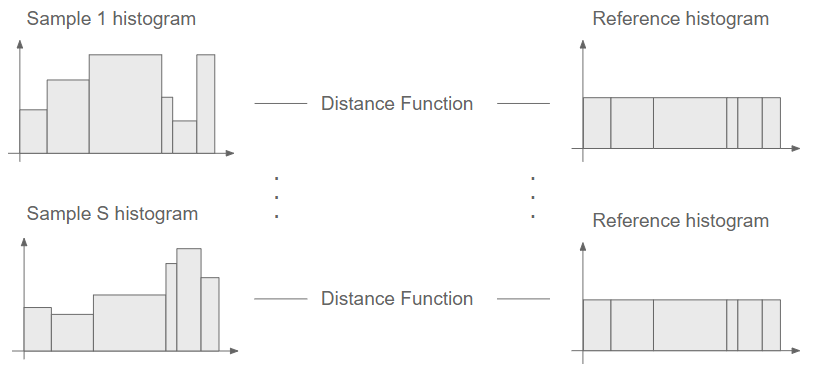
\includegraphics[scale=0.4]{figures/compute-sample-distances.png}
      \caption[Compute as many distance values as samples]{Compute as many distance values as samples, one for each sample-reference histogram pair}
      \label{fig:compute-sample-distances}
    \end{center}
\end{figure}

For each feature, we end up with \textit{S} distance values. These values are distance measurements between random samples of data and the reference period. Hence, we claim we now know the distribution of expected distance values. Given a new distance value measured between another random window and the reference window, we can compute its probability and produce alerts if below a certain threshold. Note that the histograms for each sample are EMA-like histograms (as detailed in Section \ref{sec:ema-hist}) just like the sliding window histogram. This ensures a certain degree of fidelity in the test we make in streaming because we measure the divergence between a random sample of data (our streaming histogram or any of the sample's histogram) and the reference one.


It is important to understand why we want to know the distribution of divergence values instead of just thresholding the divergence value itself. For instance, given the JSD value varies between 0 and 1, why not just set to alert if the measured JSD value is 0.7? The reason is that a divergence value may fall on different percentiles for different features. In other words, the same \textit{i-th} percentile will correspond to a different divergence value for different features. Consider the following left and right-skewed distance distributions represented by Figures \ref{fig:skewed-left-distro} and \ref{fig:skewed-right-distro}, respectively. 

\begin{figure}[!htb]
    \begin{center}
      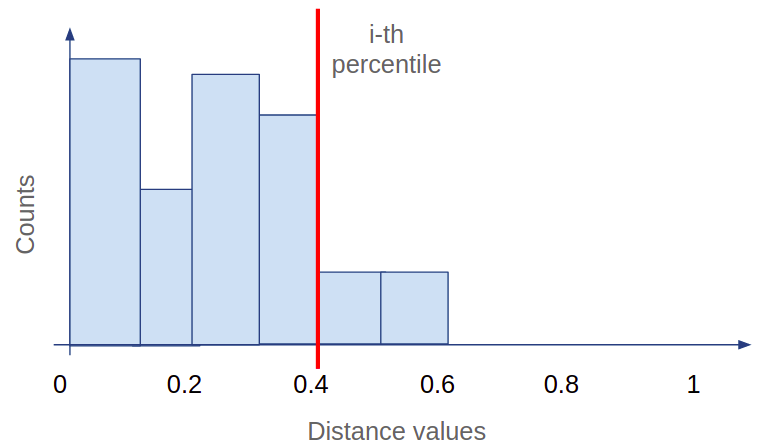
\includegraphics[scale=0.4]{figures/skewed-left-distro.png}
      \caption[]{Left skewed distribution of distance values}
      \label{fig:skewed-left-distro}
    \end{center}
\end{figure}

\begin{figure}[!htb]
    \begin{center}
      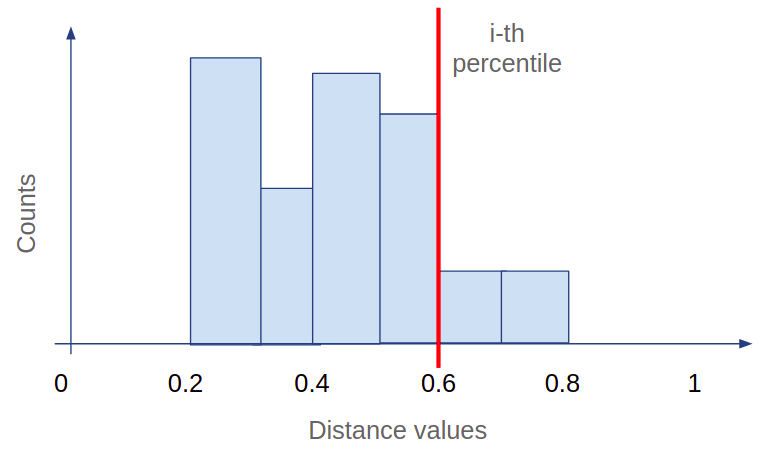
\includegraphics[scale=0.4]{figures/skewed-right-distro.png}
      \caption[]{Right skewed distribution of distance values}
      \label{fig:skewed-right-distro}
    \end{center}
\end{figure}

Let's assume Figure \ref{fig:skewed-left-distro} 's histogram encodes the distribution of expected distance values for a feature \textit{x1} and Figure \ref{fig:skewed-right-distro} does the same but for a feature \textit{x2}. Setting a user-defined threshold of \textit{$\alpha$=0.6} for both features would yield very different results. For feature \textit{x1} we would be reporting distance values above the 100th-percentile which would not be the case for feature \textit{x2}. Instead what we aim to do is know this distribution so that we can define our threshold as a percentile and not a hard-coded distance constant. For instance, in this case, we would define the threshold to be the \textit{i}-th percentile, which would correspond to a threshold value of 0.4 for feature \textit{x1} and 0.6 for feature \textit{x2}.

Hard-coding a threshold value to be used for all features is cumbersome, impractical and error-prone. The distance threshold must be computed based on the distribution of distances.


\subsubsection*{Burn-in period at system initialization}
When we boot up our system in the streaming phase we initially have empty histogram aggregations. The period of time where you discard the alerts produced by the system until it processes enough data to produce accurate reports is commonly denoted as the burn-in period. To avoid this burn-in period we propose that the sliding window approximate histogram aggregation for each feature is initialized using the last sample's histogram for that feature.

\subsubsection*{Batch phase artifacts}
For each feature, by the end of the batch phase, we have a reference histogram, a list of distance values that represents its distribution and the last sample's histogram to be used as a burn-in period for the sliding window or target histogram.

\subsection{Streaming phase} \label{sec:stream-phase}
\textcolor{red}{TODO: add some pseudocode}

In the streaming or online phase, the system will process event by event in a true sliding window fashion (recall Section \ref{sec:windows}) and perform a change detection test periodically. This phase makes use of all of the batch phase artifacts, namely, for each feature, the reference histogram, the distribution of distance values and the last sample's histogram.

For each feature, we initialize the histogram we will approximately maintain with the last sample's data, from the batch phase. Then, for each incoming event and for each of the event's features, we update our streaming approximate histogram for that feature by adding the new value and then "cutting a slice" from the top of the histogram bars to simulate eviction, as described in Section \ref{sec:ema-hist}. This is all we do, regarding event processing.

Periodically, we perform a multi-feature change detection test. The test is done by first computing the distance between the reference histogram for a feature \textit{x} and the sliding window histogram of feature \textit{x}. This distance value is then tested against the known distribution of distance values for feature \textit{x}. In other words, we test to see the percentile of the computed distance in the distribution of distance values and alert if above a certain percentile --- \textit{e.g.} the 99th-percentile. When we perform the test, for each feature \textit{x}, we are computing the percentile of the distance measured between the reference and sliding window histogram aggregations. The probability value or \textit{p-value} of a distance value is 

\[\textit{p-value\textsubscript{distance\textsubscript{x}}} = 1 - percentile(\textit{distance\textsubscript{x}})\]

Hence, if we set to alert states that have 1\% or less probability to happen, we raise an alert for distance values above the 99th-percentile or \textit{p-value} = 0.01. Generally speaking, we alert a feature \textit{x} as divergent at a given timestamp if for a given probability threshold $\alpha$:

\[ \textit{percentile(distance\textsubscript{x})} > 1 - \alpha \]

or

\begin{equation}
    \label{eq:alert-test}
    \textit{p-value\textsubscript{distance\textsubscript{x}}} < \alpha
\end{equation}

\subsubsection*{Multiple Test Correction} \label{sec:multi-test}
Note that we periodically apply this test (Equation \ref{eq:alert-test}) for each feature, effectively repeating the analysis. When considering several hypotheses, the problem of multiplicity arises: the more hypotheses are checked, the higher the probability of obtaining false positives. In other words, when repeating a test multiple times the multiple test problem arises which states that the more inferences are made, the more likely erroneous inferences are to occur. In the literature, many multiple test correction methods are proposed, but we opt to use the Holm-Bonferroni multiple test correction. The Holm-Bonferroni method is one of many approaches for controlling the so called Family-Wise Error Rate \textit{(FWER)} by adjusting the rejection criteria for each hypothesis.


\subsubsection*{Holm-Bonferroni Correction} \label{sec:holmbonferroni}
The Holm-Bonferroni correction takes Equation \ref{eq:alert-test} and corrects the right-side threshold $\alpha$ for each feature. This correction is done by dividing the threshold $\alpha$ by a correction factor, as described below.

First, we compute the \textit{p-value} of each feature. We then order our features by \textit{p-value}, in ascending order. Next, starting from the first feature, the one with the smallest \textit{p-value}, and proceeding until the end of the list of features, we check if

\[  \textit{p-value\textsubscript{distance\textsubscript{x}}} < \alpha / (\textit{m} - \textit{k}) \]

with $\alpha$ as the probability to reject the null hypothesis, \textit{m} as the number of hypotheses to test, in our case the number of features and corresponding \textit{p-values} and \textit{k} as the 0-based index of the current feature. We stop at the first feature that fails this test, and every feature processed up until this one is considered to be a divergent feature and alerts are raised.

\subsection{Final remarks}

\subsubsection*{Optimal number of samples}
In Section \ref{sec:sampling-batch} we stated we made \textit{S} samples in the batch phase. But what is the optimal number of samples to make? How can we mathematically derive a formula for the number of samples to make and avoid \textit{ad hoc} user-defined constants?

We are performing one test for each feature, hence we perform \textit{n\textsubscript{features}} tests. We apply a multiple test correction on the tests performed and want to set the Family Wise Error Rate \textit{(FWER)} to $\alpha$. In other words, we want to alert deviations for the full set of tests globally that have probability $\alpha$ < 1\%, for example.

We use the Holm-Bonferroni correction and, for each feature, we need to reliably estimate the upper tail of the distribution which corresponds to the \textit{$\alpha$ / n\textsubscript{features}} region. Each sample we do translates into a distance value and the collection of these data points builds the distribution of distance values. We want to be sure that the number of samples \textit{S} that we do generates enough distance points to have a high probability of having one or more points in the upper tail region. To that end, we define the probability of not having at least one point in the upper tail of the distance distribution as $\gamma$. 

\textcolor{red}{SEE MODEL MONITORING PAPER} We can then show that the optimal number of samples \textit{S} to make is

\begin{equation}
    \label{eq:optimal-n-samples}
    \textit{S} = \frac{\log\gamma}{log(1 - \frac{\alpha}{n\textsubscript{features}})}
\end{equation}

\subsubsection*{Distribution Divergence Statistical Tests} \label{sec:whyjsds}

We used the Jensen-Shannon Divergence (JSD) but....

\textcolor{red}{Talk about wassertein, kolomogrov, why JSD...}
